\begin{center}
    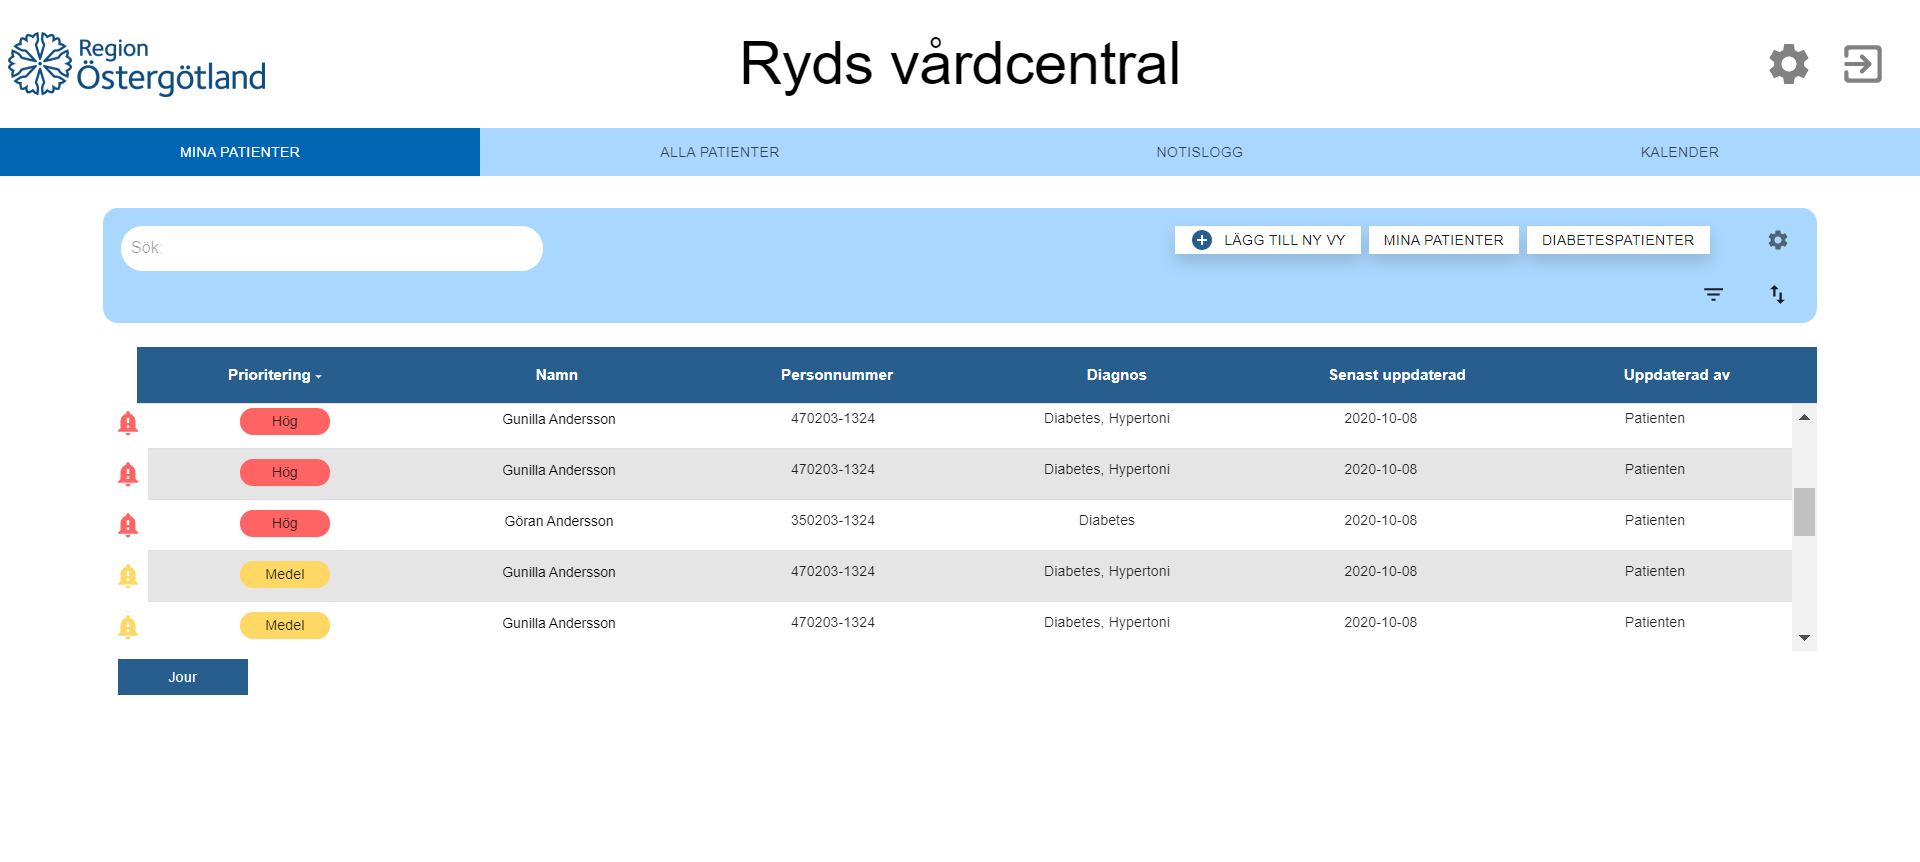
\includegraphics[width=\linewidth]{images/My_patiens_image.png}
    \captionof{figure}{My patients}
    \label{fig:figures}
\end{center}
Shows a table of all patients in the system connected to the operation (verksamhet) you are logged in to. There is an possibility to search for specific patients, filter, sort and modify the list the list. To see more about a specific patient the patients name is clicked and you are moved to the single patient's page.

By clicking on the "Jour" button at the bottom of the page a list of the doctors on call is shown, with telephone number and name.

To modify the list the gear symbol at the top right in the search bar is clicked and then in the pop-up window which appears choose the attributes wanted by ticking the associated checkbox and clicking on "Spara" (save).

To sort the list after a specific attribute the two arrows at the mid right in the search bar is clicked and then clicking on the wished attribute to sort the list after. 

To filter the table the reverse pyramid of lines at the bottom right in the search bar is clicked. A pop-up window appears, where the filters are chosen. The pop-up window looks exactly the same as the one for creating a new view which is further described below. 

There are a ability to add new views and save filters, for example one for women over 60 which has diabetes. It is possible to add up to 7 save filters. To add a filter you start by clicking "+Lägg till ny vy". A pop-up window then appears which is further described below. 

When a filter or view is active a button named "Rensa filter" shows up. By clicking on it the active filter or view is removed. 
\\

\begin{center}
    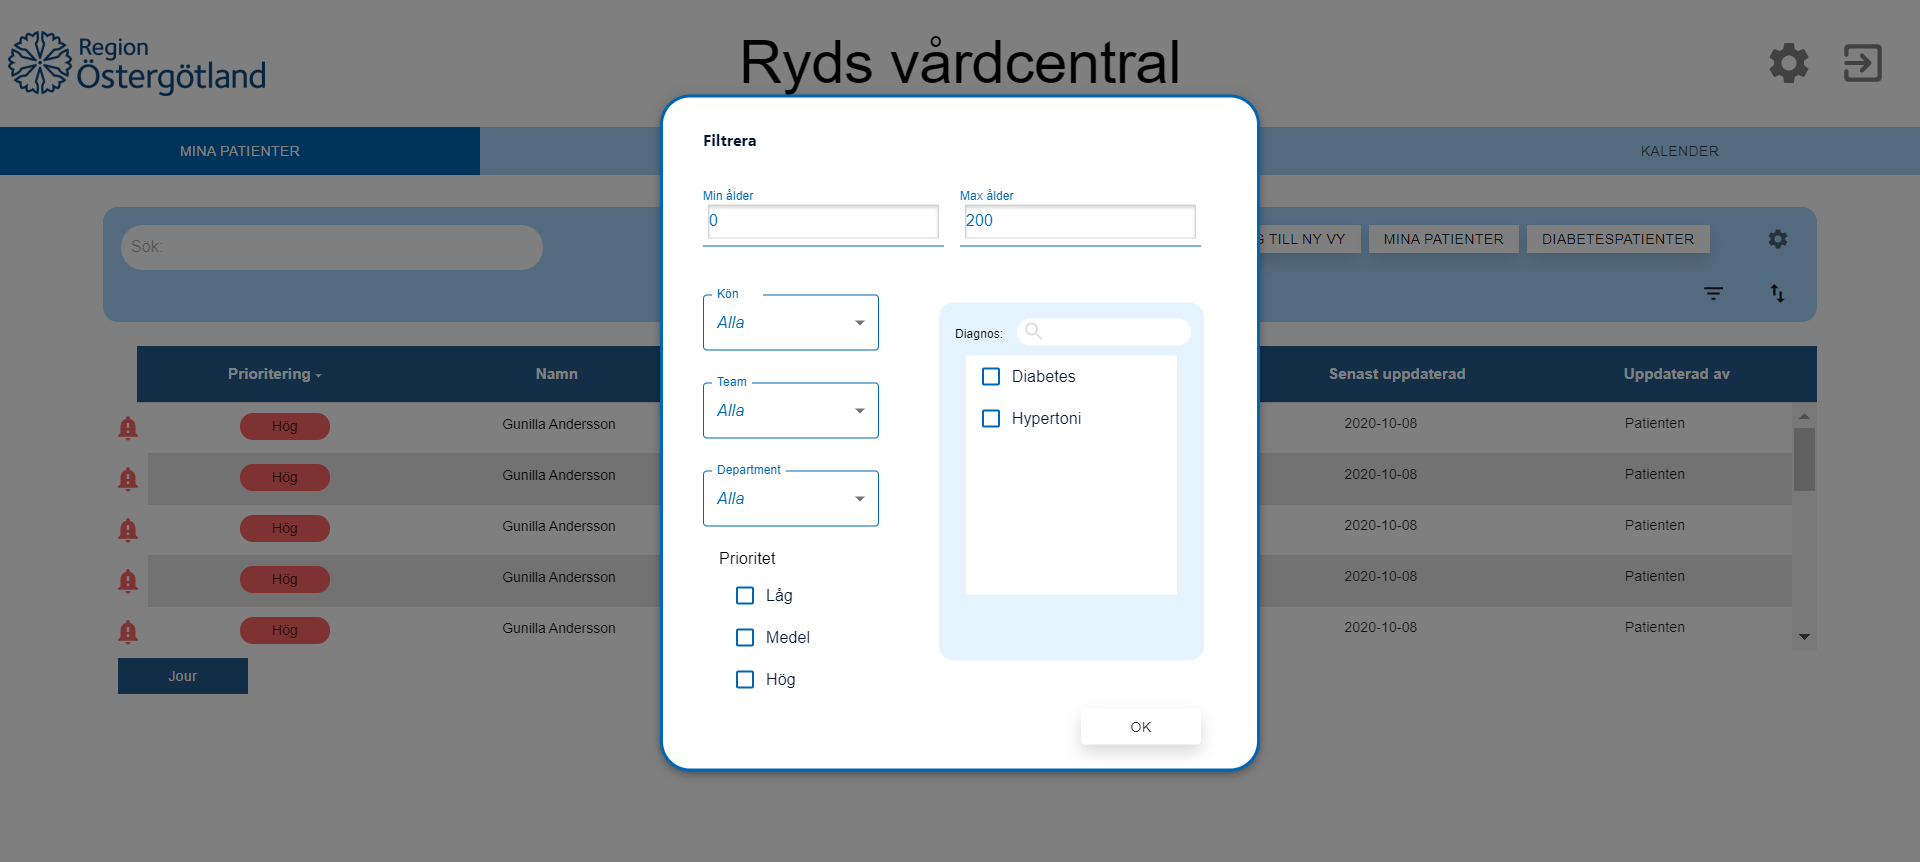
\includegraphics[width=\linewidth]{images/Add_new_view_image.png}
    \captionof{figure}{Add view}
    \label{fig:figures}
\end{center}
The pop-up window which appears when creating a new view consists of a number of attributes which can be set according to preferences. To move on click on the button "OK". To quit, just click somewhere outside the pop-up window.
\\
\begin{center}
    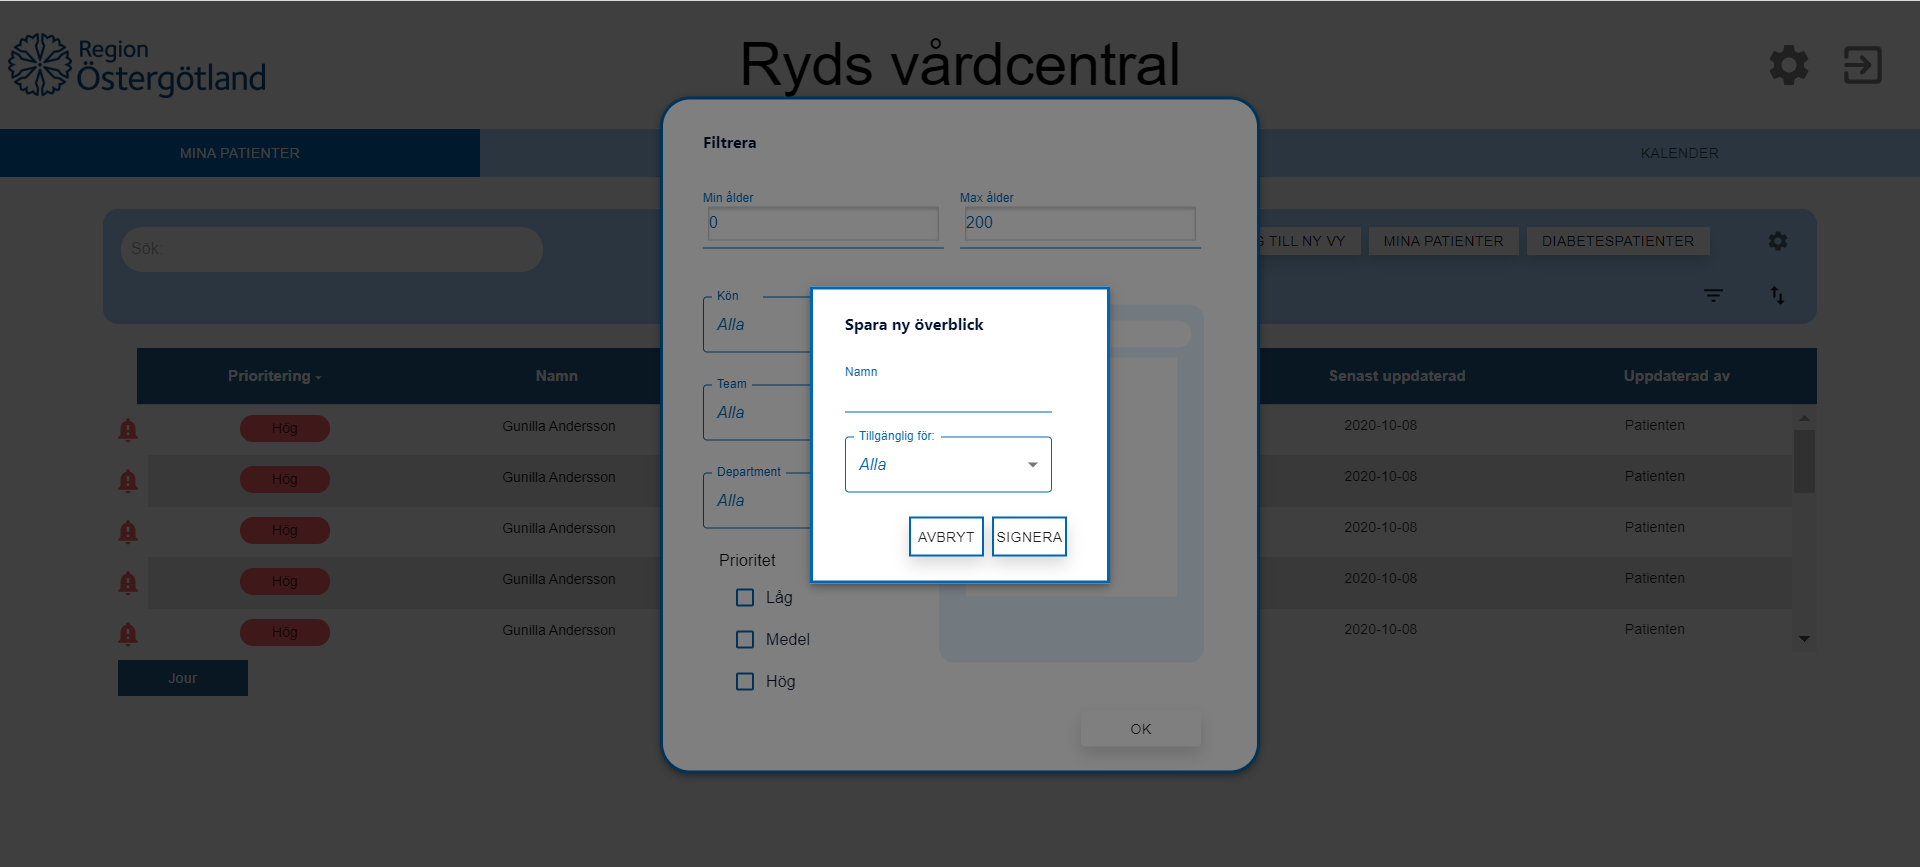
\includegraphics[width=\linewidth]{images/Save_new_view_image.png}
    \captionof{figure}{Save view}
    \label{fig:figures}
\end{center}
When preferences are chosen and clicked "OK" in the pop-up window another pop-up window appears with some further info that needs to be filled in. To finish click the "Kvittera" button. If clicking the "Avbryt" button you are moved back to the previous pop-up window.
\\
